% Fluxograma dos experimentos.
% Para o artigo (template IEEE, duas colunas): copie o bloco figure* para o .tex
% do artigo e adicione \usepackage{tikz} e \usetikzlibrary{positioning,arrows.meta}
% no preâmbulo. Este arquivo também compila sozinho para conferir o desenho.
\documentclass{article}
\usepackage[a4paper,landscape,margin=1.5cm]{geometry}
\usepackage[utf8]{inputenc}
\usepackage{tikz}
\usetikzlibrary{positioning,arrows.meta}

\begin{document}

\begin{figure*}[t]
\centering
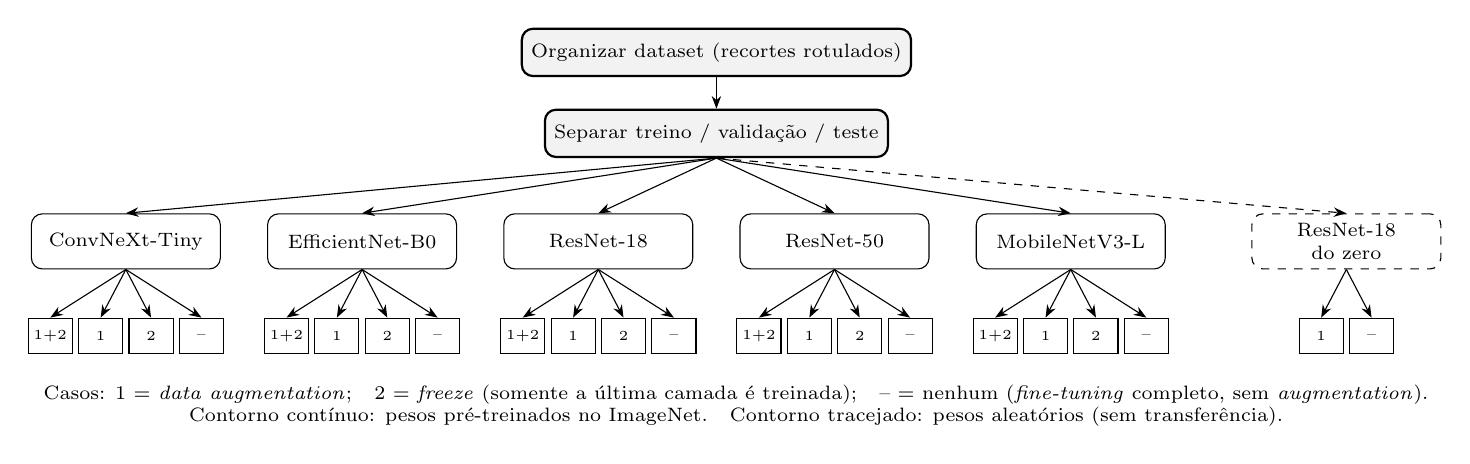
\begin{tikzpicture}[
    font=\scriptsize,
    >={Stealth[length=1.6mm]},
    etapa/.style={draw, rounded corners, thick, align=center, minimum height=6mm, fill=gray!10},
    rede/.style={draw, rounded corners, align=center, minimum width=24mm, minimum height=7mm},
    caso/.style={draw, align=center, minimum width=5.6mm, minimum height=4.5mm, inner sep=1pt, font=\tiny},
    base/.style={rede, dashed},
]
% etapas de preparação
\node[etapa] (org) at (75mm, 0) {Organizar dataset (recortes rotulados)};
\node[etapa, below=4mm of org] (split) {Separar treino / validação / teste};
\draw[->] (org) -- (split);

% redes: 5 com transfer learning (ImageNet) + linha de base do zero
\foreach \r/\txt/\x in {convnext/ConvNeXt-Tiny/0, effnet/EfficientNet-B0/30,
                        r18/ResNet-18/60, r50/ResNet-50/90, mobile/MobileNetV3-L/120} {
    \node[rede] (\r) at (\x mm, -24mm) {\txt};
    \draw[->] (split.south) -- (\r.north);
    \foreach \c/\lab/\dx in {a/1+2/-9.6, b/1/-3.2, c/2/3.2, d/--/9.6} {
        \node[caso] (\r-\c) at (\x mm + \dx mm, -36mm) {\lab};
        \draw[->] (\r.south) -- (\r-\c.north);
    }
}
\node[base] (scratch) at (155mm, -24mm) {ResNet-18\\do zero};
\draw[->, dashed] (split.south) -- (scratch.north);
\foreach \c/\lab/\dx in {b/1/-3.2, d/--/3.2} {
    \node[caso] (scratch-\c) at (155mm + \dx mm, -36mm) {\lab};
    \draw[->] (scratch.south) -- (scratch-\c.north);
}

% legenda
\node[anchor=north, align=center, font=\scriptsize] at (77.5mm, -41mm)
    {Casos: 1 = \textit{data augmentation};\quad 2 = \textit{freeze} (somente a última camada é treinada);\quad
     -- = nenhum (\textit{fine-tuning} completo, sem \textit{augmentation}).\\
     Contorno contínuo: pesos pré-treinados no ImageNet.\quad Contorno tracejado: pesos aleatórios (sem transferência).};
\end{tikzpicture}
\caption{Fluxo dos experimentos: cinco arquiteturas pré-treinadas avaliadas em quatro casos cada,
mais uma linha de base treinada do zero.}
\label{fig:fluxo}
\end{figure*}

\end{document}
